\documentclass[preprint]{elsarticle}
\usepackage[utf8]{inputenc}
\usepackage[numbers]{natbib}
\bibliographystyle{abbrvnat}
\usepackage{graphicx}
\usepackage{float}
\usepackage{wrapfig}
\usepackage[export]{adjustbox}
%% Use the option review to obtain double line spacing
%% \documentclass[preprint,review,12pt]{elsarticle}

%% Use the options 1p,twocolumn; 3p; 3p,twocolumn; 5p; or 5p,twocolumn
%% for a journal layout:
%% \documentclass[final,1p,times]{elsarticle}
%% \documentclass[final,1p,times,twocolumn]{elsarticle}
%% \documentclass[final,3p,times]{elsarticle}
%% \documentclass[final,3p,times,twocolumn]{elsarticle}
%% \documentclass[final,5p,times]{elsarticle}
%% \documentclass[final,5p,times,twocolumn]{elsarticle}

%% if you use PostScript figures in your article
%% use the graphics package for simple commands
%% \usepackage{graphics}
%% or use the graphicx package for more complicated commands
%% \usepackage{graphicx}
%% or use the epsfig package if you prefer to use the old commands
%% \usepackage{epsfig}

%% The amssymb package provides various useful mathematical symbols
\usepackage{amssymb}
%% The amsthm package provides extended theorem environments
%% \usepackage{amsthm}

%% The lineno packages adds line numbers. Start line numbering with
%% \begin{linenumbers}, end it with \end{linenumbers}. Or switch it on
%% for the whole article with \linenumbers after \end{frontmatter}.
%%\usepackage{lineno}

%% natbib.sty is loaded by default. However, natbib options can be
%% provided with \biboptions{...} command. Following options are
%% valid:

%%   round  -  round parentheses are used (default)
%%   square -  square brackets are used   [option]
%%   curly  -  curly braces are used      {option}
%%   angle  -  angle brackets are used    <option>
%%   semicolon  -  multiple citations separated by semi-colon
%%   colon  - same as semicolon, an earlier confusion
%%   comma  -  separated by comma
%%   numbers-  selects numerical citations
%%   super  -  numerical citations as superscripts
%%   sort   -  sorts multiple citations according to order in ref. list
%%   sort&compress   -  like sort, but also compresses numerical citations
%%   compress - compresses without sorting
%%
%% \biboptions{comma,round}

% \biboptions{}
\usepackage{mathtools}

\usepackage[subpreambles=true]{standalone}


\begin{document}

\begin{frontmatter}

%% Title, authors and addresses

%% use the tnoteref command within \title for footnotes;
%% use the tnotetext command for the associated footnote;
%% use the fnref command within \author or \address for footnotes;
%% use the fntext command for the associated footnote;
%% use the corref command within \author for corresponding author footnotes;
%% use the cortext command for the associated footnote;
%% use the ead command for the email address,
%% and the form \ead[url] for the home page:
%%
%% \title{Title\tnoteref{label1}}
%% \tnotetext[label1]{}
%% \author{Name\corref{cor1}\fnref{label2}}
%% \ead{email address}
%% \ead[url]{home page}
%% \fntext[label2]{}
%% \cortext[cor1]{}
%% \address{Address\fnref{label3}}
%% \fntext[label3]{}

\title{Approche hybride pour résoudre le problème du Bin Packing}

%% use optional labels to link authors explicitly to addresses:
%% \author[label1,label2]{<author name>}
%% \address[label1]{<address>}
%% \address[label2]{<address>}

\author{BACHI Yasmine, MIHOUBI LamiaZohra , MOUSSAOUI Meroua, NOUALI Sarah, SAADI Khaoula}

\address{Ecole nationale Supérieure d'Informatique -ESI-Alger}
\date{26 juin 2020}
\begin{abstract}
%% Text of abstract
L’objectif du problème du bin packing (BPP) est de trouver le nombre minimal de boîtes nécessaire pour ranger un ensemble de n objets ayant des tailles connues, en respectant la capacité de chaque boîte. Ce problème est parmis les problèmes NP-difficile. Dans cet article, on propose un algorithme génétique  hybride utilisant le recuit simulé. Les résultats expérimentaux   ont montré l’efficacité de notre hybridation dans l’amélioration de la qualité de solution de l’algorithme génétique pour les classes 1 et 2 du benchmark Scholl. \end{abstract}

\begin{keyword}
%% keywords here, in the form: keyword \sep keyword
Bin packing \sep hybridation \sep AG \sep recuit simulé \sep WOA \sep ILWOA 
%% MSC codes here, in the form: \MSC code \sep code
%% or \MSC[2008] code \sep code (2000 is the default)

\end{keyword}

\end{frontmatter}

%%
%% Start line numbering here if you want
%%
%%\linenumbers

%% main text
\section{Introduction}
\label{S:1}

Le problème du bin packing à une dimension (BPP) est défini comme suit, étant donné un nombre illimité de boîtes avec une capacité fixe C, et un ensemble de n objets, chacun ayant un poid spécifique 0<wi<C, on cherche à ranger les n objets dans un nombre minimal de boîte, tout en respectant la capacité C. 


\subsection{Algorithme génétique (AG)}
L’algorithme génétique est une heuristique de recherche initialement proposée par Holland [1] qui imite le processus de sélection naturelle.Elle appartient à la plus grande classe d'algorithmes évolutionnaires (EA), qui génèrent des solutions en utilisant des techniques inspirées de l'évolution naturelle, telles que la mutation, la sélection et le croisement.

La figure suivante représente les étapes de fonctionnement de notre AG, avec la spécification des méthodes utilisées pour implémenter chaque étape. 

\begin{figure}[!h]
    \centering
    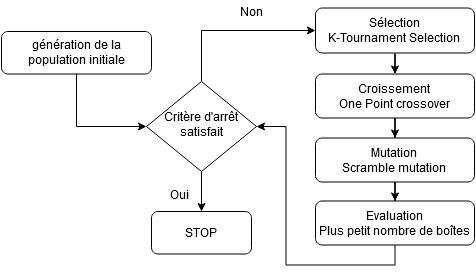
\includegraphics[scale=0.6]{./figures/AG schema.png}
    \caption{Processus de AG }
    \label{fig:agschema}
\end{figure}
Les algorithmes génétiques sont connus par leur Rapidité et facilité d’utilisation. 
En effet, le AG est parmis les métaheuristiques les plus rapides, de plus, si la la représentation vectorielle de l'individu est correcte, nous pouvons trouver une solution sans un travail d'analyse approfondi. Par contre, cette métaheuristique ne trouve pas toujours l’optimum et peut se retrouver avec le problème d’optimum local. 

\subsection{Le Recuit Simulé (SA)}
Le recuit simulé est un algorithme de recherche locale initialement introduit par Kirkpatrick et al \cite{kirk} qui simule la fusion et le refroidissement dans le traitement des métaux. Le recuit simulé est généralement implémenté pour rechercher une solution optimale sur une petite zone, même s'il est parfois aussi performant que AG dans certains cas \cite{Alkhateeb}.
Cette métaheuristique sophistiquée empêche d'être piégé dans les minima locaux à l'aide d'un moteur de recherche aléatoire exprimé en termes de chaîne de Markov. Elle introduit des changements dans la solution pour améliorer la fonction objectif, mais conserve également des solutions qui, malgré les moins bonnes performances, répondent à certains critères. Mais l’un des inconvénients du recuit simulé est son temps d'exécution élevé. 

\subsection{Hybridation}
Pour surmonter les inconvénients  de GA et SA, plusieurs études proposent une hybridation entre les deux.
Junghans et Darde \cite{Junghans} comparent entre AG et AG hybride avec SA modifiée (MSA).
Le SA utilisé dans leur expérience a été modifié pour contrôler la réduction de la température.
Ils ont découvert que le GA-MSA hybride offre une fiabilité plus élevée que le AG.
Une autre recherche menée par Chen et Shahandashti dans \cite{Chen} qui compare également le GA, SA, un hybride de GA-SA et MSA, où ils ont constaté que le GA-SA hybride est plus performante que AG, SA et MSA. \\
Dans cet article, nous avons hybridé le GA-SA avec quatres scénarios, à savoir le AG-RS hybride,le AGH-RS , le AG-2RS et le AG-MIX, Le schéma hybride AG-RS consiste à obtenir la meilleure solution en AG et à l'utiliser comme population initiale en SA,
le AGH-RS utilise le même processus sauf que AG à été initialisé par plusieurs heuristiques.Le schema AG-2RS  consiste à inclure SA dans le AG après l’étape de mutation, et améliorer la solution de AG par le SA à nouveau. finalement le schéma AG-MIX utilise le même processus que AG-2RS en initialisant le AG par plusieurs heuristiques. 
D’autres schémas ont été implémenté et serons inclus dans la comparaison, on cite le WOA-RS  et le ILWOA-RS qui sont une hybridation de haut niveau des métaheuristiques WOA et ILWOA avec le recuit simulé.

 
 \subsection{Organisation du papier}
 On va tout d’abord définir le problème du bin packing, sa représentation mathématique, par la suite on présentera nos schémas hybrides proposés. Finalement, des résultats expérimentaux sont donnés et une comparaison des schémas hybrides est effectuée  dans [ num], suivi d’une conclusion.

\section{Formulation du problème}
\subsection{Défénition du problème}
Le problème du bin packing à une dimension (BPP) est défini comme suit, étant donné un nombre illimité de boîtes avec une capacité fixe C, et un ensemble de n objets, chacun ayant un poid spécifique 0<wi<C, on cherche à ranger les n objets dans un nombre minimal de boîte, tout en respectant la capacité C. 

\subsection{Formulation mathématique}
Etant donné \(m\) boites de capacité \(C\) et \(n\) articles de volume \(v_i\) chacun. \\
    Soient: 
    \[ x_{ij} =
        \begin{cases}
            1  & \quad \text{article } j \text{ rangé dans la boîte } i \\
            0  & \quad \text{sinon } 
        \end{cases}
    \]
    \[ y_i =
    \begin{cases}
        1  & \quad \text{boîte } i \text{ utilisée } \\
        0  & \quad \text{sinon } 
    \end{cases}
    \]

La formulation du problème donne ainsi le programme linéaire suivant
\[(PN)
    \begin{cases}
        Z(min) = \displaystyle\sum_{i=1}^{m} y_i \\
        \displaystyle\sum_{i=1}^{m} x_{ij}  = 1 \\
        \displaystyle\sum_{j=1}^{n} v_j x_{ij} \le C y_i \\
        y_i \in \{0,1\} \\
        x_{ij} \in \{0,1\} 
    \end{cases}
\]  
La première contrainte signifie qu’un article j ne peut être placé qu’en une seule boite
La deuxième fait qu’on ne dépasse pas la taille d’une boite lors du rangement

\section{L'approche hybride proposée}
Pour le schéma de l’hybridation proposé dans cet article,il s’agit d’une hybridation  classifiée selon la taxonomie de talbi comme suit 
\textbf{HRH globale, généraliste }, et qui utilise l'algorithme génétique comme méthode révolutionnaire,
suivie par un  Recuit Simulé pour l'intensification des résultats de ce dernier.

\subsection{Encodage de la solution}
\subsubsection{Solution du bin packing}
La solution sera représentée par: 
\begin{itemize}
    \item une liste de boîtes, où la boîte est représenté par une liste des objets qui y sont rangés, et l’objet est représenté par un entier désignant son poids.  poids des objets qui y sont rangés, ainsi que le nombre de boîtes utilisées, ce qui représente le coût de la solution, et nous permettra  d’évaluer la performance de l’algorithme en terme de la qualité de la solution.
    \begin{figure}[h!]
        \centering
        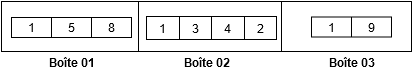
\includegraphics[scale=0.6]{./figures/Untitled Diagram(6).png}
    \end{figure}
    \item Le nombre de boîtes utilisées, ce qui représente le coût de la solution, et nous permettra  d’évaluer la performance de l’algorithme en terme de la qualité de la solution.

\end{itemize}
\subsubsection{Représentation chromosomique}
Pour cette implémentation de l’AG, nous allons utiliser une nouvelle représentation chromosomique, proposée dans \cite{Mohamadi}, On représente une solution du Bin packing comme suit: 
\begin{itemize}
    \item On suppose qu’on a ‘n’ articles à ranger donc on utilisera n boîtes au maximum.
    \item Chaque boîte est composée de  “n” cellules, où chaque cellule ne peut contenir qu’un seul article.
    \item Chaque cellule à un numéro unique dans la solution.
    \item Si la cellule de l’ordre i de la boite j est remplie par un objet, alors on aura plus le droit de ranger un objet dans toutes les cellules de l’ordre i des autres boites.
    \item La cellule “zero” contient le nombre de boîtes utilisés dans cette solution.
\end{itemize}
Dans le chromosome , on ne garde trace que des numéros de cellules où les objets sont stockés, donc la taille du chromosome sera de 1+n, où n est le nombre d'objets à ranger.

\textbf{Exemple:} Supposons que nous avons quatre objets (n=4) de poids 2, 2, 4 et 4 respectivement, affectés à trois cases (c0=3)  comme indiqué ci-dessous :
\begin{figure}[H]
\end{figure}
Le chromosome correspondant est le suivant : 
\begin{figure}[H]
\end{figure}
Ceci signifie que le nombre de boîtes utilisé est 3, le premier objet est rangé dans la première cellule(boîte 1) , le deuxième objet est rangé dans la 2ème cellule (boîte 1), le 3ème objet est rangé dans la 7ème cellule ( boîte 2), et le 4ème objet est rangé dans la 12ème cellule ( boîte 3) .

\subsection{L'hybridation AG-RS}
Une hybridation entre AG et RS permet à AG d'explorer un énorme espace de recherche et à RS d'exploiter des zones de recherche locales. Le RS commence généralement par une solution initiale aléatoire, dans la solution proposée, la meilleure solution de AG est utilisée comme configuration initiale, et le Recuit simulé va se charger de l’intensification de cette dernière, où il utilise un processus de recherche d'une solution optimale globale dans l'espace de la solution, grâce à son aspect aléatoire, et qui a été prouvé de guider l’algorithme vers l’optimum global. 
Donc, le GA est puissant pour obtenir une solution presque optimale sur la zone de recherche large tandis que SA est utile pour rechercher une solution dans la zone de recherche étroite.\cite{Gusti}

\medskip

\bibliography{Samples}

\end{document}

%%\begin{table}[h]
%%\centering
%%\begin{tabular}{l l l}
%%\hline
%%\textbf{Treatments} & \textbf{Response 1} & \textbf{Response 2}\\
%%\hline
%%Treatment 1 & 0.0003262 & 0.562 \\
%%Treatment 2 & 0.0015681 & 0.910 \\
%%Treatment 3 & 0.0009271 & 0.296 \\
%%\hline
%%\end{tabular}
%%\caption{Table caption}
%%\end{table}

